% Packages & Document Configurations
\documentclass[onecolumn]{NobArticle}
\usepackage[utf8]{inputenc}
\usepackage{listings}
\usepackage{xcolor}
\usepackage{multicol}
\usepackage{float}
\usepackage[table,xcdraw]{xcolor}
\usepackage{hyperref}

\definecolor{codegreen}{rgb}{0,0.6,0}
\definecolor{codegray}{rgb}{0.5,0.5,0.5}
\definecolor{codepurple}{rgb}{0.58,0,0.82}
\definecolor{backcolour}{rgb}{0.95,0.95,0.92}

\lstdefinestyle{mystyle}{
    backgroundcolor=\color{backcolour},   
    commentstyle=\color{codegreen},
    keywordstyle=\color{magenta},
    numberstyle=\tiny\color{codegray},
    stringstyle=\color{codepurple},
    basicstyle=\ttfamily\footnotesize,
    breakatwhitespace=false,         
    breaklines=true,                 
    captionpos=b,                    
    keepspaces=true,                 
    numbers=left,                    
    numbersep=5pt,                  
    showspaces=false,                
    showstringspaces=false,
    showtabs=false,                  
    tabsize=2
}

\lstset{style=mystyle}


% Title
\title{Comparative Analysis of Different Prompting Methods for Large Language Model}

% Authors
\author{
    Hyoyeon Lee\textsuperscript{1}
}

% Affiliations
\date{
    \textsuperscript{\textbf{1}}
    School of Computer Science, University of Bristol
}

\begin{document}

\small
\maketitle
\section{Introduction}
This document presents a comparative analysis of various prompting techniques based on their memory usage and execution time when applied to Gemini-Flash 1.5. The study evaluates three distinct methods: one-shot prompting, Chain-of-Thought (CoT) prompting, and few-shots prompting. Notably, the current implementation does not incorporate counterexamples from the CBMC (C Bounded Model Checker) with the new prompts. Instead, it uses 'simple restart' method which uses the same prompt and relies on the possibility of obtaining a different response from the LLM than previously returned. Additionally, the number of reattempt has been restricted to three to avoid the hallucination of the LLM and endless reiteration of the software. This comparison aims to provide insights into the efficiency and performance of each prompting strategy, thereby guiding the appropriate usage of prompting methods.

\vspace{11pt}
\section{Experimental Setup}
In this section, I define the overall procedure of the experiment and its environment settings. For the exact prompt, check \hyperref[sec:prompting_methods]{Section 3}.

\subsection{Implementation}
I tested three different prompting methods to input code into Gemini Flash-1.5, receive the generated response, and verify its correctness using CBMC. The prompt has been refined from looping until it individually checks all proof harness functions generated to create a new function, 'combined\_proof\_harness()', to verify its correctness all at once. This approach reduced the running time as it removed the need of creating a separate JSON file of CBMC results per every proof harness functions. A 'simple restart' method has been applied when reattempting to query the LLM.

\subsection{LLM}
Gemini Flash 1.5 has been used for generating proof harness functions, where its temperature has been fixed to default temperature of 0.25 to ensure its determinism. Other hyperparameters have been set to default as well.

\subsection{CBMC}
CBMC 6.0.1 has been used to verify the correctness of generated proof harness functions. Identical CBMC command '\texttt{cbmc FILE\_NAME.c --function combined\_proof\_harness --no-standard-checks --no-malloc-may-fail --verbosity 8 --unwind 3 --trace --json-ui}' has been used for every prompting method. As the updated version of CBMC was released, new flags were used to restore the default value of the previous version of CBMC.


\subsection{Benchmarks}
The benchmarks were collected from real-world datasets on Kaggle, primarily related to LeetCode problems. All programs were written in C, using only standard libraries to avoid errors. The programs primarily focus on algorithmic and arithmetic operations, and they employ a variety of data structures, including numeric values, pointers, arrays, and structs.


\begin{table}[H]
    \centering
    \begin{tabular}{c c c c c c c c}
    \hline
    \textbf{Prompt Method} & \textbf{Project} & \textbf{Success} & \textbf{\#Iteration} & \textbf{Runtime} & \textbf{Memory Usage} & \textbf{LoC} & \textbf{\#Functions}
    \\ \hline
    
    One shot & prompt.c & True & 2 & 28.7236 & 90093 & 42 & 5 &
    Few shots & prompt.c & False & 3 & 42.7236 & 318866 & 42 & 5 &
    CoT & prompt.c & True & 1 & 4.8829 & 81507 & 42 & 5
    \\ \hline
    \end{tabular}
\end{table}

\vspace{-0.6cm} % Adjust the space if necessary
\begin{center}
\textbf{Table 1: Benchmark details and format}
\end{center}

Details on the benchmark are provided in Table 1. The verification result, indicated by 'Success', is marked as 'True' for successful verification from the CBMC and 'False' otherwise. The total number of iterations for each project is listed under '\#Iteration'. The iteration count is limited to three; projects that reached the maximum iteration number without 'True' success result are considered unsuccessful. The total runtime and memory usage are reported by 'Runtime' and 'Memory Usage' in seconds and bytes, respectively. The runtime and memory usage have not been averaged to better reflect the LLM's capability to generate correct and safe C codes in a given number of iteration.


\vspace{11pt}
\section{Prompting Methods}
\label{sec:prompting_methods}
The following are the three different sample prompt formats: one-shot prompting, few-shots prompting, and Chain-of-Thought prompting, to query Gemini Flash 1.5 for generating proof harness functions. New constraint regarding library declarations has been added due to frequent failures in proof harness function generation, 'assert.h' in particular.

\subsection{One-shot Prompting}
\begin{lstlisting}[language=, caption=One-shot Prompting Format]
  # Preamble
    You are given a C program. We need to create a proof harness function.
    # Code generation example - You are given three examples.

    Q: Write a method "void proof_harness_withdraw()" that tests method withdraw below for all possible inputs.

    // Define the Account structure
    struct Account {{
        unsigned short bal;
    }};

    // Function to withdraw an amount from an account
    void withdraw(struct Account *account, unsigned short amount) {{ 
        unsigned short de = account->bal;
        account->bal = de - amount; 
    }}

    A:
    struct Account {{
    unsigned short bal;
        }};
    
    
    void withdraw(struct Account *account, unsigned short amount) {{
        unsigned short de = account->bal;
        account->bal = de - amount;
    }}
    
    void proof_harness_withdraw() {{
        struct Account *account = (struct Account *)malloc(sizeof(struct Account));
        __CPROVER_assume(account != NULL);  // Ensure account is not NULL
    
        unsigned short amount;
    
        __CPROVER_assume(account->bal >= 0);
        __CPROVER_assume(amount > 0);
        __CPROVER_assume(account->bal >= amount);
    
        unsigned short initial_balance = account->bal;
    
        withdraw(account, amount);
        assert(account->bal == initial_balance - amount);
    
        free(account);
    }}


    # Instruction
    Give me a proof harness code of the below C code.

    # Query 
    Q: Write method "void proof_harness_{{function_name}}()" that tests every methods including 'main()' 
    below for all possible inputs. Then write a method "void combined_proof_harness()" that calls every other proof 
    harness methods generated. 
    
    {query_code}.

    # Constraints
    Here are some constraints that you should respect:
    - Give me only the translated code, don't add explanations or anything else. 
    - Use only safe C.
    - Do not use custom generics. # fuzzer limitation
    - Do not remove any code from the original code you have received.
    - Ensure that all libraries needed, including <assert.h>, are declared at the beginning of the code.

    
\end{lstlisting}


\subsection{Few-shots prompting}
% \subsection{Prompt Format}

\begin{lstlisting}[language =, caption= Prompt Format]

  # Preamble
    You are given a C program. We need to create a proof harness function.
    
    # Code generation example
    ## Example 1
        Q: Write a method "void proof_harness_withdraw()" that tests method withdraw below for all possible inputs.
        // Define the Account structure
        struct Account {{
            unsigned short bal;
        }};
    
        // Function to withdraw an amount from an account
        void withdraw(struct Account *account, unsigned short amount) {{ 
            unsigned short de = account->bal;
            account->bal = de - amount; 
        }}
    
        A:
        struct Account {{
        unsigned short bal;
            }};
        
        
        void withdraw(struct Account *account, unsigned short amount) {{
            unsigned short de = account->bal;
            account->bal = de - amount;
        }}
        
        void proof_harness_withdraw() {{
            struct Account *account = (struct Account *)malloc(sizeof(struct Account));
            __CPROVER_assume(account != NULL);  // Ensure account is not NULL
        
            unsigned short amount;
        
            __CPROVER_assume(account->bal >= 0);
            __CPROVER_assume(amount > 0);
            __CPROVER_assume(account->bal >= amount);
        
            unsigned short initial_balance = account->bal;
        
            withdraw(account, amount);
            assert(account->bal == initial_balance - amount);
        
            free(account);
        }}
	## end Example 1
		
	## Example 2
		Q: Write method "void proof_harness_{{function_name}}()" that tests every methods below for all possible inputs.
         #include <stdio.h>
		#include <stdlib.h>
		
		struct node{{
		    struct node *leftNode;
		    int data;
		    struct node *rightNode;
		}};
		
		struct node *newNode(int data){{
		    struct node *node = (struct node *)malloc(sizeof(struct node));
		    node->leftNode = NULL;
		    node->data = data; node->rightNode = NULL;
		    return node;
		}}
		
		int main(void){{
		    return 0;
		}}
		
		A: 
		#include <stdio.h>
		#include <stdlib.h>
		#include <assert.h>
		
		struct node{{
		    struct node *leftNode;
		    int data;
		    struct node *rightNode;
		}};
		
		struct node *newNode(int data){{
		    struct node *node = (struct node *)malloc(sizeof(struct node));
		    node->leftNode = NULL;
		    node->data = data; node->rightNode = NULL;
		    return node;
		}}
		
		int main(void){{
		    return 0;
		}}
		
		void proof_harness_newNode() {{
		    int data;
		    __CPROVER_assume(data >= 0);
		    __CPROVER_assume(data <= 2147483647);
		    struct node *node = newNode(data);
		    assert(node != NULL);
		    assert(node->leftNode == NULL);
		    assert(node->data == data);
		    assert(node->rightNode == NULL);
		    free(node);
		}}

	## end Example 2
		
	## Example 3
		 Q: Write method "void proof_harness_{{function_name}}()" that tests every methods below for all possible inputs.
    
         #include <stdio.h>

		struct node{{
		    struct node *leftNode;
		    int data;
		    struct node *rightNode;
		}};
		
		void inOrderTraversal(struct node *node){{
		    if (node == NULL) return;
		    inOrderTraversal(node->leftNode);
		    printf("\t%d\t", node->data);
		    inOrderTraversal(node->rightNode);
		}}
		
		void preOrderTraversal(struct node *node){{
		    if (node == NULL) return;
		    printf("\t%d\t", node->data);
		    preOrderTraversal(node->leftNode);
		    preOrderTraversal(node->rightNode);
		}}
		
		void postOrderTraversal(struct node *node){{
		    if (node == NULL) return;
		    postOrderTraversal(node->leftNode);
		    postOrderTraversal(node->rightNode);
		    printf("\t%d\t", node->data);
		}}
		
		int main(void){{
		    return 0;
		}}
		
		A: 
		
		#include <stdio.h>
        #include <assert.h>

		struct node{{
		    struct node *leftNode;
		    int data;
		    struct node *rightNode;
		}};
		
		void inOrderTraversal(struct node *node){{
		    if (node == NULL) return;
		    inOrderTraversal(node->leftNode);
		    printf("\t%d\t", node->data);
		    inOrderTraversal(node->rightNode);
		}}
		
		void preOrderTraversal(struct node *node){{
		    if (node == NULL) return;
		    printf("\t%d\t", node->data);
		    preOrderTraversal(node->leftNode);
		    preOrderTraversal(node->rightNode);
		}}
		
		void postOrderTraversal(struct node *node){{
		    if (node == NULL) return;
		    postOrderTraversal(node->leftNode);
		    postOrderTraversal(node->rightNode);
		    printf("\t%d\t", node->data);
		}}
		
		int main(void){{
		    return 0;
		}}
		
		void proof_harness_inOrderTraversal() {{
		    struct node *node = (struct node *)malloc(sizeof(struct node));
		    __CPROVER_assume(node != NULL);
		    node->leftNode = NULL;
		    node->rightNode = NULL;
		    __CPROVER_assume(node->data >= 0 && node->data <= 100);
		    inOrderTraversal(node);
		    free(node);
		}}
		
		void proof_harness_preOrderTraversal() {{
		    struct node *node = (struct node *)malloc(sizeof(struct node));
		    __CPROVER_assume(node != NULL);
		    node->leftNode = NULL;
		    node->rightNode = NULL;
		    __CPROVER_assume(node->data >= 0 && node->data <= 100);
		    preOrderTraversal(node);
		    free(node);
		}}
		
		void proof_harness_postOrderTraversal() {{
		    struct node *node = (struct node *)malloc(sizeof(struct node));
		    __CPROVER_assume(node != NULL);
		    node->leftNode = NULL;
		    node->rightNode = NULL;
		    __CPROVER_assume(node->data >= 0 && node->data <= 100);
		    postOrderTraversal(node);
		    free(node);
		}}
		
	## end Example 3
				
# Instruction
    Give me a proof harness code of the below C code.

# Query
    Q: Write method "void proof_harness_{{function_name}}()" that tests every methods including 'main()' 
    below for all possible inputs. Then write a method "void combined_proof_harness()" that calls every other proof 
    harness methods generated. 
    
    {query_code}

    # Constraints
    Here are some constraints that you should respect:
    - Give me only the translated code, don't add explanations or anything else. 
    - Use only safe C.
    - Do not use custom generics. # fuzzer limitation
    - Do not remove any code from the original code you have received.
    - Ensure that all libraries needed, including <assert.h>, are declared at the beginning of the code.
    
\end{lstlisting}

The prompt has been set to include three examples to prevent excessive length and minimise the risk of hallucinations from the LLM. As it will be demonstrated in the results, for few-shot prompting, which is the longest prompt format, longer codes significantly increase the likelihood of hallucinations and failure rates.

\vspace{11pt}
\subsection{Chain-of-Thought (CoT)}
\begin{lstlisting}[caption=Generated Proof Harness Function]
  # Preamble
    You are given a C program. We need to create a proof harness function.
    # Code generation example
    Q: Write a method "void proof_harness_withdraw()" that tests method withdraw below for all possible inputs.

    // Define the Account structure
    struct Account {{
        unsigned short bal;
    }};

    // Function to withdraw an amount from an account
    void withdraw(struct Account *account, unsigned short amount) {{ 
        unsigned short de = account->bal;
        account->bal = de - amount; 
    }}

    A: You first identify which functions there are. In this case, we have a single function called 'withdraw'. Since 
    withdraw is a function that needs to be tested, we create a proof_harness_withdraw function for this purpose and 
    implement to test the correctness of the function 'withdraw'.
    
    struct Account {{
    unsigned short bal;
        }};
    
    
    void withdraw(struct Account *account, unsigned short amount) {{
        unsigned short de = account->bal;
        account->bal = de - amount;
    }}
    
    void proof_harness_withdraw() {{
        struct Account *account = (struct Account *)malloc(sizeof(struct Account));
        __CPROVER_assume(account != NULL);  // Ensure account is not NULL
    
        unsigned short amount;
    
        __CPROVER_assume(account->bal >= 0);
        __CPROVER_assume(amount > 0);
        __CPROVER_assume(account->bal >= amount);
    
        unsigned short initial_balance = account->bal;
    
        withdraw(account, amount);
        assert(account->bal == initial_balance - amount);
    
        free(account);
    }}
    

    # Instruction
    Give me a proof harness code of the below C code.

    # Query
    Q: Write method "void proof_harness_{{function_name}}()" that tests every methods including 'main()' 
    below for all possible inputs. Then write a method "void combined_proof_harness()" that calls every other proof 
    harness methods generated.
    
    {query_code}

    # Constraints
    Here are some constraints that you should respect:
    - Give me only the translated code, don't add explanations or anything else. 
    - Use only safe C.
    - Do not use custom generics. # fuzzer limitation
    - Do not remove any code from the original code you have received.
    - Ensure that <assert.h> is declared when using assert. 
    """ 
\end{lstlisting}


\section{Results}
\quad I run an experiment for each of the three prompts for a total of 366 proof harness functions generation and correctness verification experiment. The input C programs were validated to ensure them using safe C codes by identifying those that returned conversion errors and the pre-processing them accordingly.  The results have been rounded to four decimal places. 


\subsection{Success Rate with regards to Line of Code and number of functions}

\begin{figure}[H]
    \centering
    \begin{minipage}{0.48\linewidth}
        \centering
        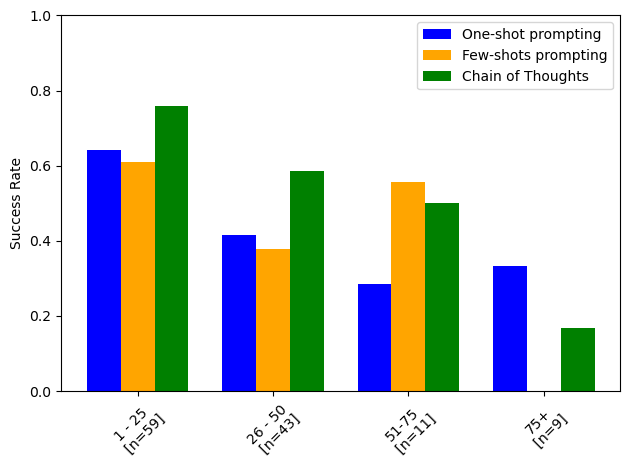
\includegraphics[width=\linewidth]{LineofCode_successrate.png}
        \textbf{Figure 1: Success Rate of prompting methods grouped by Line of Code}
        \label{fig:lineofcode-successrate}
    \end{minipage}
    \hfill
    \begin{minipage}{0.48\linewidth}
        \centering
        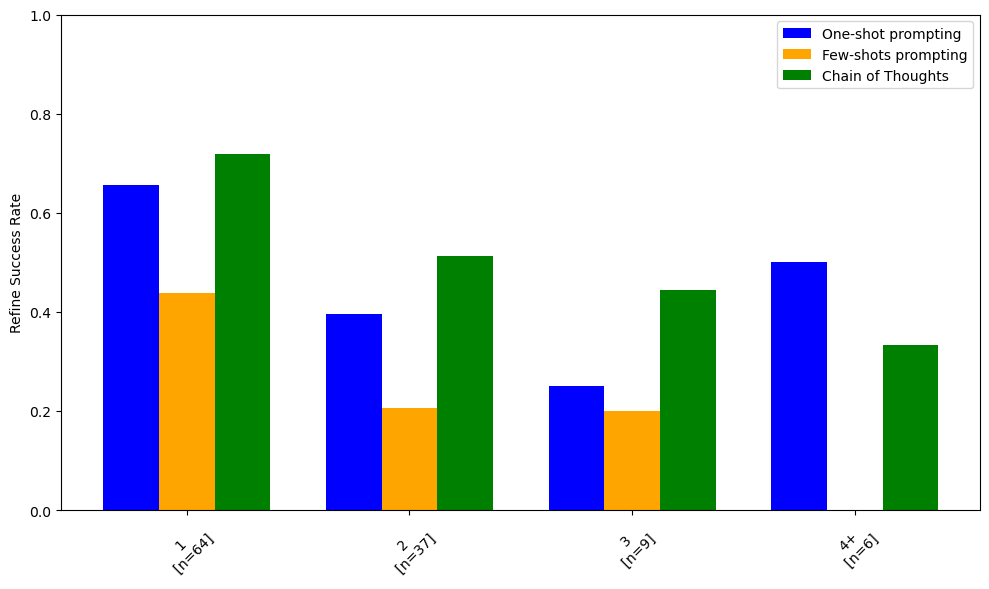
\includegraphics[width=\linewidth]{Function number_success rate.png}
        \textbf{Figure 2: Success rate for each prompt strategies on benchmarks grouped by number of functions}
        \label{fig:function-number-successrate}
    \end{minipage}
\end{figure}


\vspace{-0.1cm}
\begin{table}[h]
\centering
\begin{tabular}{|c|c|c|c|c|}
\hline
\textbf{Prompting methods \textbackslash{} LoC} & \textbf{1 $\sim$ 25} & \textbf{26 - 50} & \textbf{51-75} & \textbf{75+} \\ \hline
\textbf{One-shot prompting}                    & 35.9375                                 & 58.5366                            & 71.4286                       & 66.6667                       \\ \hline
\textbf{Few-shots prompting}                   & 38.8889                            & 62.0690                            & 44.4444                       & 100                               \\ \hline
\textbf{Chain of Thoughts}                     & 24.0741                             & 41.4634                            & 50                                & 83.3333                       \\ \hline
\end{tabular}
    \vspace{0.2cm}
    % \vspace{-0.5cm} % Adjust the space if necessary
    \begin{center}
    \textbf{Table 2: Failure rates of prompting methods by Line of Code (percentage)}
    \end{center}
\end{table}

\begin{table}[h!]
\centering
\begin{tabular}{|c|c|c|c|c|}
\hline
\textbf{\#Functions} & \textbf{One-shot Prompting} & \textbf{Few-shots Prompting} & \textbf{CoT} & \textbf{\#Samples} \\
\hline
\textbf{1} & 65.6716 & 43.8596 & 71.8750 & 64 \\
\hline
\textbf{2} & 39.4737 & 20.5882 & 51.3514 & 37 \\
\hline
\textbf{3} & 25 & 20 & 44.4444 & 9 \\
\hline
\textbf{4+} & 50 & 0 & 33.3333 & 6 \\
\hline
\end{tabular}
    \begin{center}
    \textbf{Table 3: Failure Rates of Prompting Methods by Line of Code (percentage)}
    \end{center}
\label{table:prompting-methods}
\end{table}


\vspace{-0.3cm}
Figure 1 and Figure 2 illustrates the success rates of different prompting methods  in relation to the length of the input code, measured in lines of code and number of functions, respectively. The success rates for are presented for four ranges of code length: 1-25 lines, 26-50 lines, 51-75 lines, and 75+ lines. Additionally, Figure 2 categorises the data by the number of functions the input C program contained: a single function, two functions, three functions, and four or more functions. The results indicate a general trend where longer prompts and more extensive input code correlate with lower success rates. Specifically:
\begin{description}[font=$\bullet$\scshape\bfseries]
    \item[One-shot prompting] demonstrates a significant decrease in success rate as the line of code increase. It achieves its highest success rate of 64.06\% with the shortest code line group and drops to its lowest rate of 28.57\% within the 51-75 lines range. Regarding the number of functions, one-shot prompting shows consistent performance across different numbers of functions, with the highest success rate observed for single-function code (64.71\%) and the lowest for code with three functions (33.33\%).
    \vspace{0.2cm}
    \item[Few-shots prompting] exhibits its highest success rate of 61.11\% with 1-25 lines and the lowest with the longest line of codes. Notably, there exists an anomaly in the 51-75 lines group, where the success rate increases by approximately 18.25\% from the previous group. This indicates that the few-shots prompting performs better performance with moderately long code.  Apart from the line of code, few-shots prompting shows lower performance as the number of functions increases. Its success rate significantly drops compared to other prompting methods, with the lowest performance observed for code with four or more functions (16.67\%).

    \vspace{0.2cm}
    \item[Chain-of-Thought prompting] maintains the highest success rates among the tested prompting methods for the first three groups. Similarly to other prompting methods, the performance gradually declines for longer code, but shows a highest average success rate among all three. In terms of the number of functions, Chain-of-Thought consistently shows high performance across different function groups. Although there is a decline in success rate as the number of functions increases, Chain-of-Thought remains the most effective method compared to the others.

\end{description}

\vspace{11pt}
\subsection{Refine Success Rate}
\vspace{11pt}
\begin{table}[H]
    \centering
    \begin{tabular}{|c|c|c|}
    \hline
    \textbf{One-shot prompting}
         &  \textbf{Few-shots prompting}
         & \textbf{CoT prompting}
         \\ \hline
    5.8333 \% &  1.8692 \% & 3.7383 \%
    \\ \hline
    \end{tabular}
    \begin{center}
    \textbf{Table 3: Refine success rate}
    \end{center}
\end{table}

\quad Adopting the 'simple restart' strategy, the success rate of refined proof harness function verification was much lower than expected for all three methods. One-shot prompting showed the best ability to return valid proof harness functions, followed by Chain-of-Thoughts prompting with a 3.74\% lower success rate. The few-shots prompting method demonstrated the lowest probability of fixing bugs in its proof harness function generation.

\vspace{11pt}
\subsection{Average Runtime and Memory Usage}
\begin{figure}[H]
    \centering
    \begin{minipage}{0.48\linewidth}
        \centering
        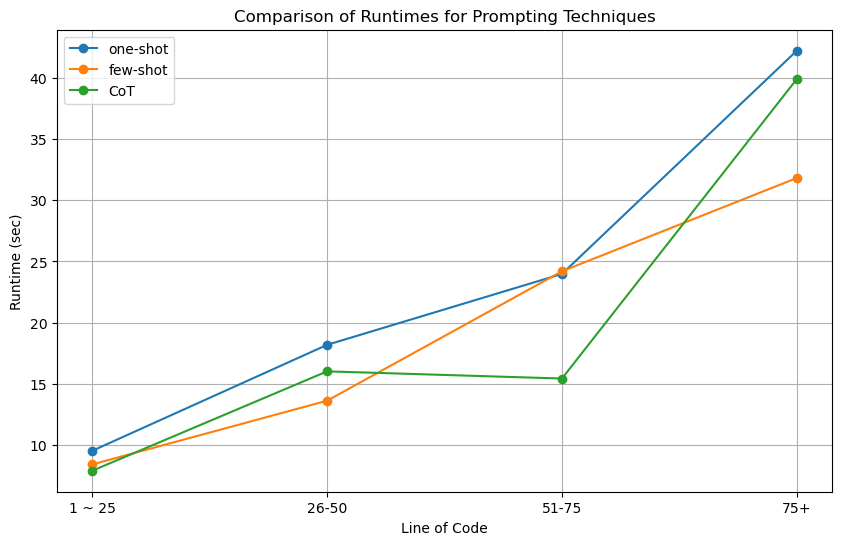
\includegraphics[width=\linewidth]{Runtime analysis.png}
         \begin{center}
        \textbf{Figure 3: Average Runtime (sec)}
    \end{center}
    \end{minipage}
    \hfill
        \begin{minipage}{0.48\linewidth}
        \centering
        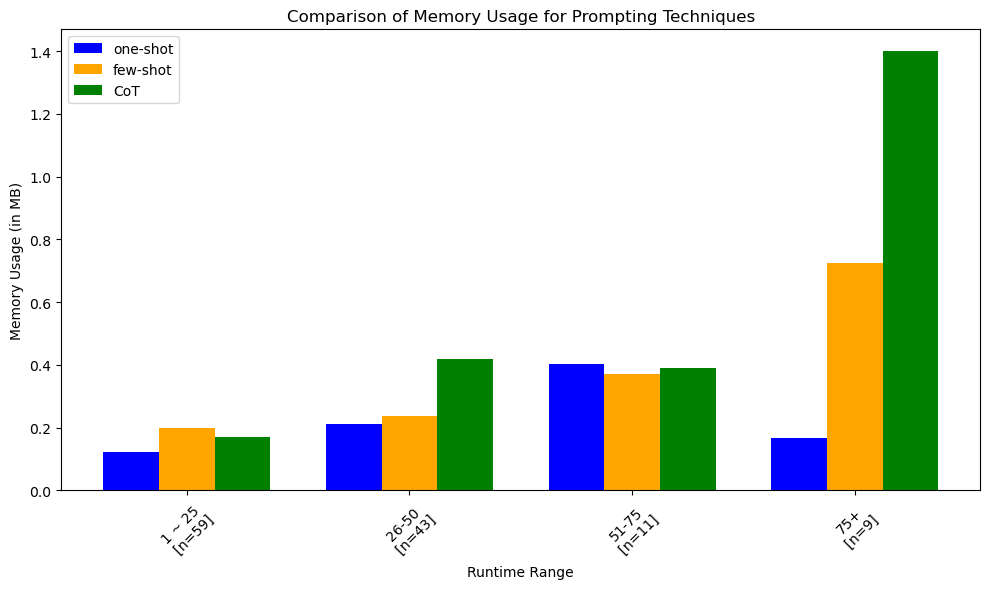
\includegraphics[width=\linewidth]{Memory Usage.png}
         \begin{center}
        \textbf{Figure 4: Average Memory Usage (MB)}
    \end{center}
    \end{minipage}
\end{figure}

\quad Before the results are delved, it must be noted that the Chain-of-Thought prompting strategy had two extremely large outliers, which caused the average runtime to increase dramatically. The runtime and memory usage figure has been extracted from the very start until the program finished its final iteration. \newline

\quad The overall average runtime increased as the length of the input code got longer, as well as the memory usage for all three prompting strategies. One-shot prompting shows a gradual increase in runtime as the line of code increases, with a significant jump for the longest code group (75+ lines). Few-shots prompting maintains a relatively stable runtime, with it showing almost a linear relationship between the line of code and the runtime. Chain-of-Thought (CoT) prompting has the shortest runtime for most code lengths but also exhibits a sharp increase for the longest code group, potentially influenced by two extreme outliers. In terms of memory usage, one-shot prompting displays the lowest memory usage across all code lengths, few-shots prompting has moderate memory usage increasing steadily with longer code, and Chain-of-Thought (CoT) prompting shows the highest memory usage, especially for the longest code group, indicating a significant increase in resource consumption.


\vspace{11pt}
\section{Conclusion}
\quad The comparative analysis of different prompting methods for proof harness function verification using Gemini Flash 1.5 reveals significant insights into their performance. One-shot prompting emerged as the most effective method in terms of both success rate and resource efficiency, although its performance notably decreased with longer lines of code and multiple functions. Chain-of-Thought prompting, despite having two large outliers that affected the average runtime, maintained a high success rate across varying code lengths and function numbers, showing consistent performance. Few-shots prompting, while relatively stable in runtime, demonstrated the lowest success rate and the highest memory usage, particularly as the code length increased. Given these results, when LLMs are not provided with feedback from previous failures, they are more likely to succeed if the input is of moderate length and contains fewer functions. The 'simple restart' strategy yielded lower-than-expected success rates for all three methods, with One-shot prompting leading, followed by Chain-of-Thought prompting, and Few-shots prompting trailing behind. Overall, these findings suggest that One-shot prompting is generally preferable for tasks requiring efficient and reliable proof harness function verification, while Chain-of-Thought prompting offers a balanced alternative, especially when runtime and memory usage are less of a concern.

\vspace{11pt}
\section{Further Discussions}
\subsection{Using Different Feedback Strategies}
\quad Since the current feedback strategy does not show commendable performance in generating valid and safe proof harness functions, trying different feedback strategies such as providing counterexamples could be considered. Incorporating counterexamples into the feedback prompt may help in guiding the model to correct its previous mistakes more effectively, potentially increasing the overall success rate and robustness of the generated proof harness functions. By leveraging more detailed and constructive feedback, it may be possible to enhance the model's learning process and improve the quality of its outputs.


\printbibliography

\end{document}
